\documentclass[11pt,a4paper]{article}
\usepackage[margin=22mm]{geometry}
\usepackage{amsmath}
\usepackage{booktabs}
\usepackage{graphicx}
\usepackage{float}
\graphicspath{{figures/}}
\setlength{\parindent}{0pt}
\setlength{\parskip}{5pt}
\renewcommand{\arraystretch}{1.22}
\setlength{\textfloatsep}{6pt}
\setlength{\intextsep}{6pt}

\begin{document}

\begin{titlepage}
\centering
\vspace*{2cm}
{\Large\textbf{ASSIGNMENT REPORT-7}}\\[0.7cm]
{\large\textbf{GMM MODELS AND PATTERN RECOGNITION}}\\[1.7cm]
\textbf{Submitted by:}\\[0.4cm]
\textbf{KARTHIKEYAN M} [26120004]\\[0.3cm]
\textbf{MIRTHULA M} [26120121]\\[1.8cm]
\textbf{Under the guidance of:}\\[0.4cm]
\textbf{HEMA ARUNACHALAM MURTHY}\\[1.5cm]
\textbf{For the subject}\\[0.4cm]
{\Large\textbf{Pattern Recognition and Machine Learning}}\\[0.3cm]
\textbf{(26AI5707)}
\vspace{2cm}

{\textbf{DEPARTMENT OF COMPUTER SCIENCE \& ENGINEERING}\\[0.3cm]
\textbf{SHIV NADAR UNIVERSITY, CHENNAI}\\[0.3cm]
\textbf{OCTOBER 2026}}
\end{titlepage}

\section*{INTRODUCTION}
This experiment is all about, we building a GMM for each class and use it to classify test data. We first use the 2 class data that we generated in Lab 6 and then work with MNIST digits given for our team with is 2, 3 and 9.

\section*{METHOD}
Primary idea of GMM is a class contain several Gaussian components:
\[
p(\mathbf{x})=\sum_{k=1}^{K}\pi_k\,\mathcal{N}(\mathbf{x};\boldsymbol{\mu}_k,\Sigma_k),
\qquad \sum_{k=1}^{K}\pi_k=1.
\]
Here, $\boldsymbol{\mu}_k$ is the component mean, $\Sigma_k$ is its covariance and $\pi_k$ is its mixture weight.

We first use K-means to initialize the parameters that is need for  GMM. EM then kicks in and starts calculating responsibilities and then updating the means, covariances and weights. For classification, we choose the class whose GMMs splits out the highest likelihood.

\section*{SYNTHETIC DATA}
Each class has 5,000 points generated out of three Gaussian components, with mixture weights $(0.5,0.3,0.2)$. We use an 80/20 train--test split and fit one three-component GMM per class.

\begin{figure}[H]
\centering
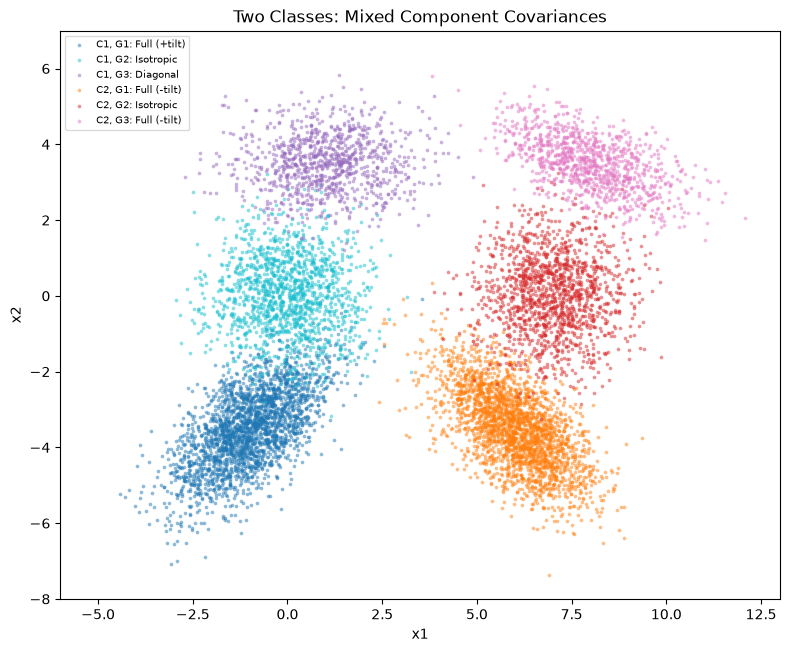
\includegraphics[width=0.45\textwidth]{mixture_data.png}
\caption{Two classes, each generated from three Gaussian components.}
\end{figure}

\textbf{Test confusion matrix}
\begin{center}
\begin{tabular}{lcc}
\toprule
 & Predicted class 1 & Predicted class 2 \\
\midrule
True class 1 & 999 & 1 \\
True class 2 & 1 & 999 \\
\bottomrule
\end{tabular}
\end{center}
\textbf{Test accuracy: 99.90\%} (1,998 correct out of 2,000).

\clearpage
\section*{MNIST DATA AND TRAINING}
Our team is assigned with digits 2, 3 and 9. Each was $28\times28$ image that gets flattened into 784 pixel values and divided by 255. We have decided to go without patching since we have the compute.

Only training images are involved to fit the parameters. We try different K values such as 3, 5 and 8 components per digit and choose the number that gives out the best development accuracy. The test set is kept aside for the final evaluation.

\begin{center}
\begin{tabular}{cr}
\toprule
Components per digit & Development accuracy \\
\midrule
3 & 96.65\% \\
5 & 96.76\% \\
\textbf{8} & \textbf{97.51\%} \\
\bottomrule
\end{tabular}
\end{center}
We select \textbf{8 components per digit}, as it gives out the highest development accuracy among the three choices.

\begin{figure}[H]
\centering
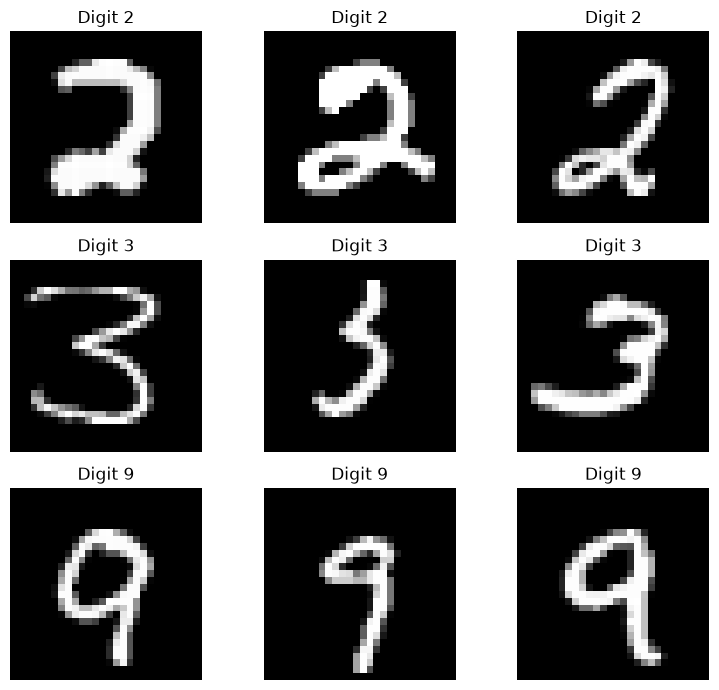
\includegraphics[width=0.60\textwidth]{mnist_samples.png}
\caption{Examples of the original MNIST images used in this experiment.}
\end{figure}

\clearpage
\section*{MNIST TEST RESULTS}
\textbf{Test accuracy: 97.57\%} (2,977 correct out of 3,051; 74 errors).

\begin{figure}[H]
\centering
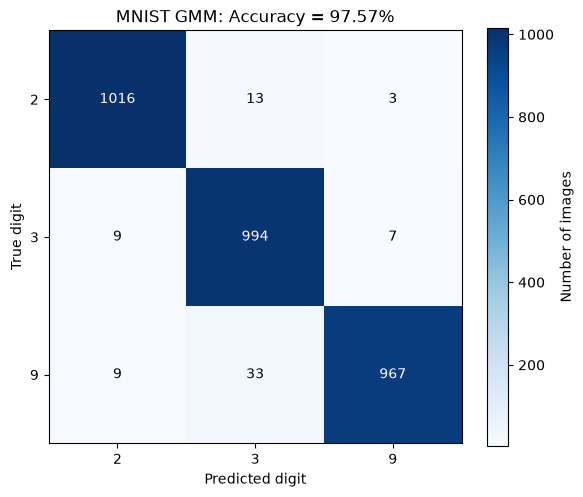
\includegraphics[width=0.55\textwidth]{mnist_confusion.png}
\caption{Confusion matrix. Rows show the actual digit and columns show the predicted digit.}
\end{figure}

\begin{figure}[H]
\centering
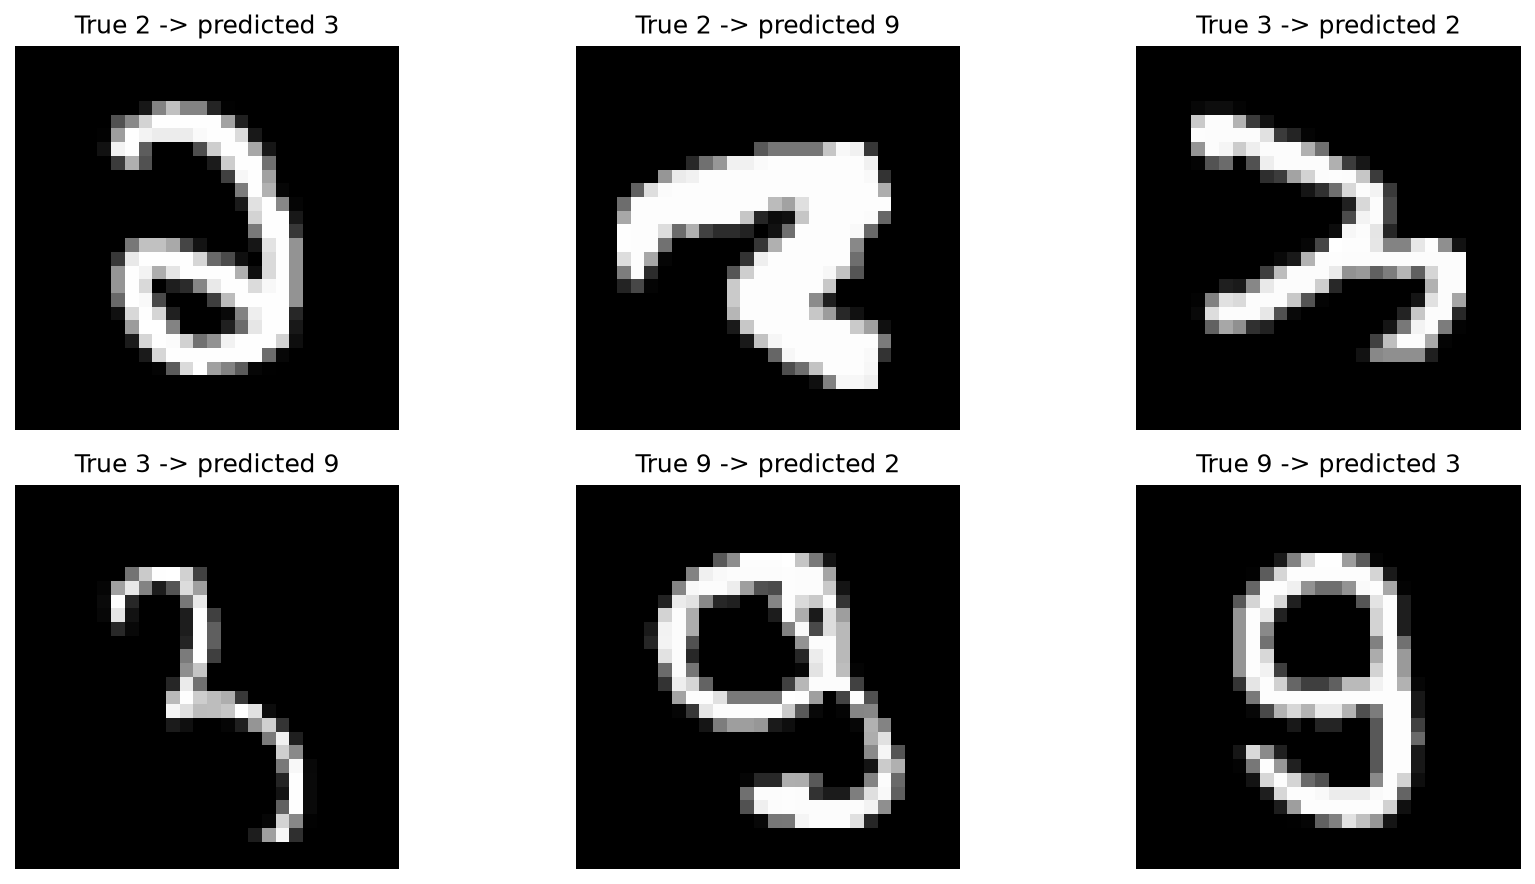
\includegraphics[width=0.94\textwidth]{mnist_errors.png}
\caption{The first misclassified test image for each actual--predicted digit pair.}
\end{figure}

Most confusions happened on 9 to 3 (33 images). These images received higher likelihood under the digit-3 GMM; We can spot similar handwritten loops and curves among the 2 digits and that may contribute to the errors.

\clearpage
\section*{LEARNED COMPONENT MEANS}
\begin{figure}[H]
\centering
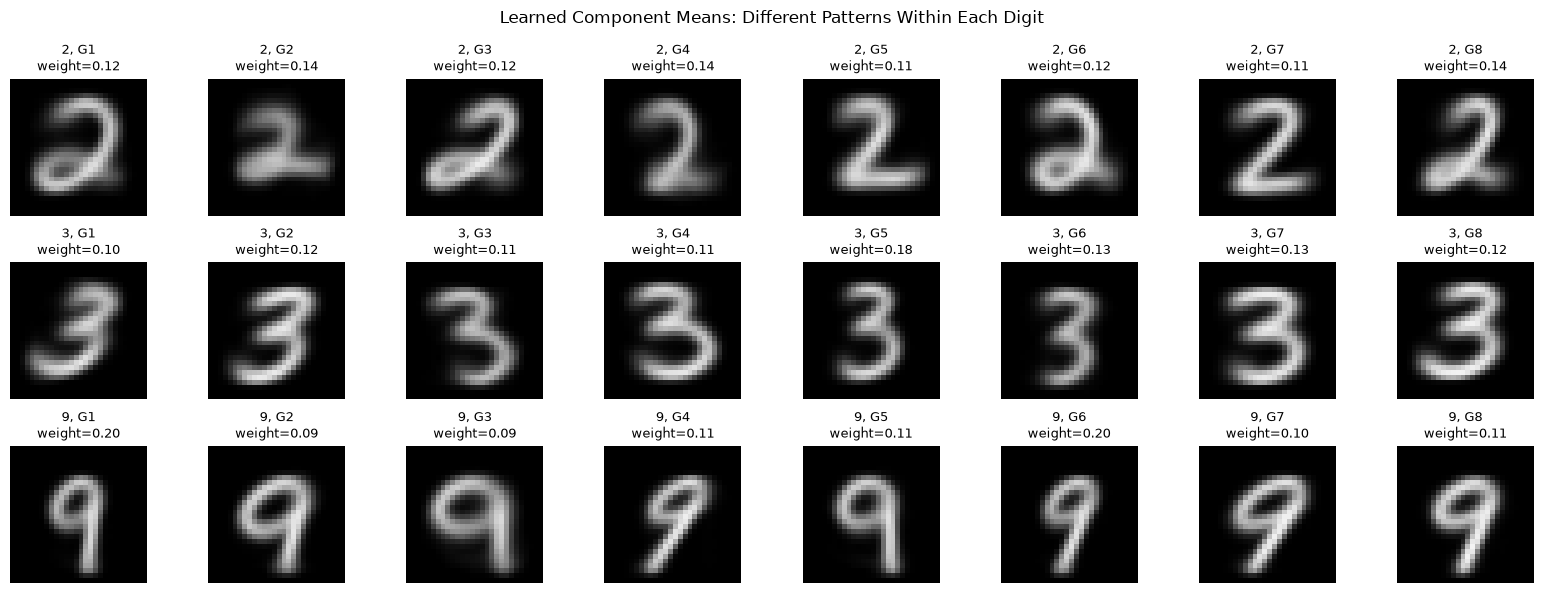
\includegraphics[width=0.98\textwidth]{mnist_component_means.png}
\caption{Learned component means for digits 2, 3 and 9.}
\end{figure}

\begin{figure}[H]
\centering
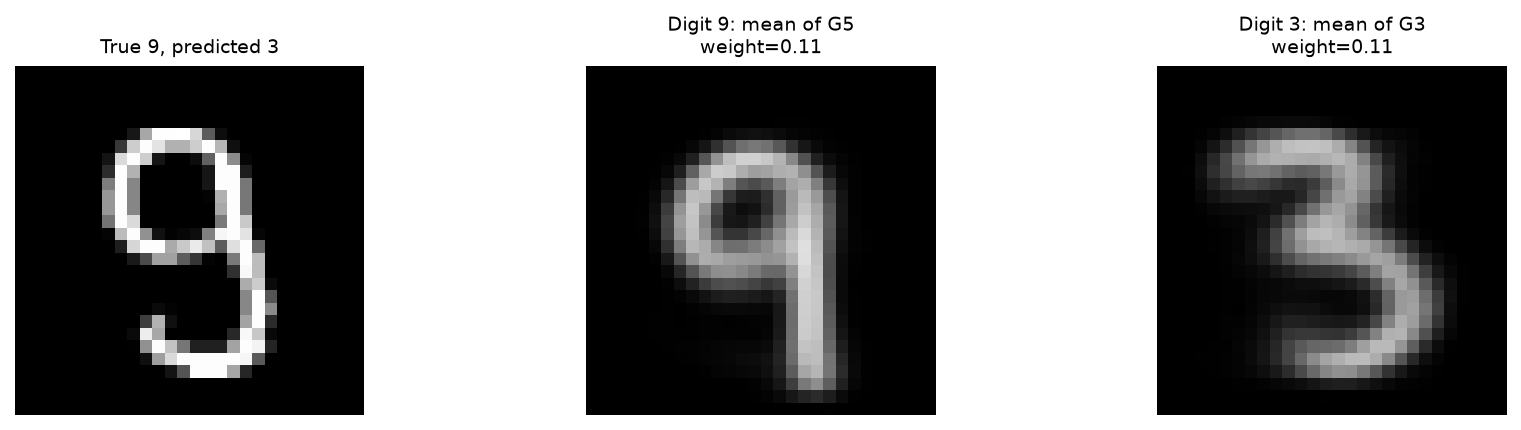
\includegraphics[width=0.96\textwidth]{mnist_component_comparison.png}
\caption{Misclassified 9 and component means from the digit-9 and digit-3 GMMs.}
\end{figure}

\section*{CONCLUSION}
The primary learning is that one GMM can represent different patterns within a class. We used 3 components per class for the synthetic data and 8 components per digit for MNIST.

\end{document}
